\chapter{\ifproject%
\ifenglish Project Structure and Methodology\else โครงสร้างและขั้นตอนการทำงาน\fi
\else%
\ifenglish Project Structure\else โครงสร้างของโครงงาน\fi
\fi
}

\makeatletter

% \renewcommand\section{\@startsection {section}{1}{\z@}%
%                                    {13.5ex \@plus -1ex \@minus -.2ex}%
%                                    {2.3ex \@plus.2ex}%
%                                    {\normalfont\large\bfseries}}

\makeatother
%\vspace{2ex}
% \titleformat{\section}{\normalfont\bfseries}{\thesection}{1em}{}
% \titlespacing*{\section}{0pt}{10ex}{0pt}

\section{โครงสร้างโดยรวมของโครงงาน (project overview) }
\begin{mypara}
    \indent โครงงานนี้เป็นระบบสนับสนุนการตัดสินใจสำหรับการวางแผนระบบขนส่งสาธารณะ 
    โดยจะจัดทำเป็นเว็บแอพลิเคชั่นสำหรับการจำลอง และมีการสรุปผลลัพธ์ที่ได้จากการจำลองในรูปแบบทางสถิติ
    ซึ่งในการทำงานของระบบนี้จะมี 4 องค์ประกอบหลักดังนี้  
\end{mypara}


\begin{figure}[H]
    \centering
    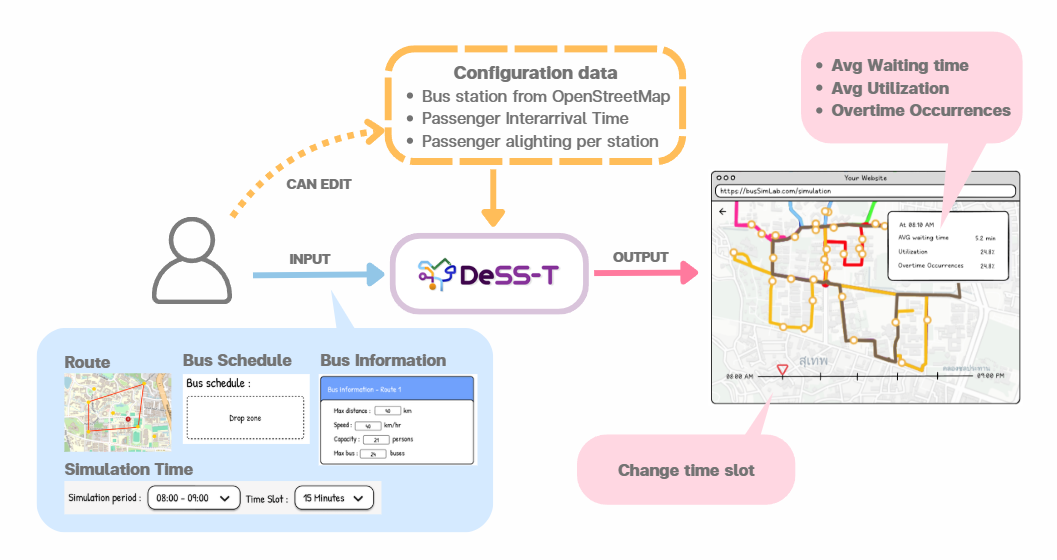
\includegraphics[width=\textwidth,height=0.9\textheight,keepaspectratio]{overview.png}
    \caption{แผนภาพโดยรวมของโครงงาน}
    \label{fig:overview}
\end{figure}

\subsection{input}
\begin{mypara}
  \indent เป็นส่วนที่รับข้อมูลจากผู้ใช้ที่จะมีการเปลี่ยนแปลงอยู่เสมอ ได้แก่ เส้นทางการให้บริการของรถในแต่ละสายบริการ 
  ตารางเวลาการออกรถ ช่วงเวลาที่ต้องการดูผลการจำลอง ข้อมูลของรถซึ่งมี ความจุผู้โดยสาร ระยะทางที่สามารถวิ่งได้สูงสุด 
  ความเร็วในการวิ่ง
\end{mypara}
\subsection{configuration data}
\begin{mypara}
  \indent เป็นส่วนของข้อมูลที่ใช้เป็นพื้นฐานในการจำลองซึ่งจะไม่ค่อยมีการเปลี่ยนแปลงบ่อย 
  ได้แก่ ข้อมูลช่วงระยะห่างของเวลาที่ผู้โดยสารแต่ละคนมาถึงที่สถานี ข้อมูลของจำนวนผู้โดยสารที่ลงจากรถในแต่ละสถานี 
  และข้อมูลที่เกี่ยวข้องกับสถานีซึ่งจะเก็บในรูปแบบของ network model ซึ่งจะมี 
  node เป็นรายชื่อสถานี และ มี edge เป็นระยะทางละหว่างแต่ละสถานี
  \end{mypara}
\subsection{simulation engine}
\begin{mypara}
  \indent เป็นส่วนที่ทำหน้าที่ในการจำลองระบบขนส่งสาธารณะตามข้อมูลที่ได้รับจากส่วน input 
  และ configuration data ซึ่งจะใช้เทคนิคการจำลองแบบเหตุการณ์ไม่ต่อเนื่อง (discrete-event simulation) 
  ในการจำลองระบบขนส่งสาธารณะ 
\end{mypara}
\subsection{output}
\begin{mypara}
  \indent เป็นส่วนที่แสดงผลลัพธ์ที่ได้จากการจำลอง โดยจะมีข้อมูล การรอเฉลี่ยของผู้โดยสาร อัตราการใช้งานของรถ 
  ซึ่งจะมีข้อมูลแสดงทั้งข้อมูลรวมทุกสถานี และข้อมูลรายละเอียดของแต่ละสถานีแยกกัน รวมถึงจะมี dashboard 
  สำหรับแสดงผลลัพธ์ในรูปแบบกราฟเพื่อให้ผู้ใช้สามารถวิเคราะห์ข้อมูลได้ง่ายขึ้น
\end{mypara}
\section{ ขั้นตอนการทำงาน (Process Overview)}
\begin{mypara}
    \indent โครงงานนี้ทำงานโดยนำข้อมูลจากผู้ใช้ (input) มาจำลองระบบขนส่งสาธารณะ 
    โดยอ้างอิงจาก configuration data ซึ่งประกอบด้วยข้อมูลหลายประเภท 
    โดยบางส่วนจะถูกนำไปสร้างเป็น distribution function เพื่อใช้ในการสุ่มพฤติกรรมของผู้โดยสาร 
    ขณะที่ข้อมูลอีกส่วนจะถูกนำมาใช้โดยตรง ใน simulation engine ซึ่งจะประมวลผลด้วย
    เทคนิคการจำลองแบบเหตุการณ์ไม่ต่อเนื่อง (discrete-event simulation) 
    เพื่อสร้างผลลัพธ์เชิงสถิติที่สะท้อนประสิทธิภาพของระบบขนส่งสาธารณะมาแสดงผลในส่วน output
\end{mypara}

\section{User Interface (UI)}
\begin{mypara}
    \indent โครงงานนี้มีการออกแบบเพื่อให้ผู้ใช้สามารถป้อนข้อมูลที่จำเป็นสำหรับ
    ารจำลองระบบขนส่งสาธารณะได้อย่างสะดวกและไม่ซับซ้อน 
    โดยข้อมูลที่มีการเปลี่ยนแปลงบ่อย จะถูกจัดให้อยู่ในส่วนของ input 
    ซึ่งสามารถเข้าถึงและแก้ไขได้ง่ายโดยไม่ต้องผ่านขั้นตอนที่ซับซ้อน 
    ส่วนข้อมูลพื้นฐานของระบบขนส่งสาธารณะ จะถูกจัดเก็บแยกเป็น configuration data 
    เพื่อให้ง่ายต่อการนำมาใช้ซ้ำ และมี workspace สำหรับการจัดการข้อมูลที่ช่วยให้ผู้ใช้สามารถ 
    clone configuration data หรือ input จากผู้อื่นมาใช้งานและปรับแก้ได้สะดวก

  \indent ในส่วนของ output ได้ออกแบบให้สามารถแสดงผลได้ทั้งมุมมองภาพรวมและ
  รายละเอียดรายสถานี เพื่อให้ผู้ใช้ตรวจสอบข้อมูลเชิงลึกได้อย่างครบถ้วน นอกจากนี้ยังมี 
  dashboard สรุปผล ที่นำเสนอข้อมูลในรูปแบบกราฟและตัวชี้วัดสำคัญ 
  เพื่อช่วยให้ผู้ใช้สามารถเปรียบเทียบและวิเคราะห์ประสิทธิภาพของระบบขนส่งสาธารณะ
  ได้อย่างสะดวกและมีประสิทธิภาพ
\end{mypara}

\subsection{การจัดกลุ่มผู้ใช้ (User Grouping)}
\begin{mypara}
\indent โครงงานนี้มีการจัดกลุ่มผู้ใช้เป็น 2 กลุ่มหลัก ได้แก่
\begin{itemize}
    \item ผู้ใช้ที่ลงทะเบียน (Registered Users): กลุ่มนี้เป็นผู้ใช้ที่สร้างบัญชีและเข้าสู่ระบบเรียบร้อยแล้ว 
    สามารถเข้าถึงฟังก์ชันทั้งหมดของระบบ สามารถบันทึกการจำลองหรือ upload ข้อมูลขึ้นไปบน workspace ได้ 
    \item ผู้ใช้ที่ไม่ได้ลงทะเบียน (Guest Users / Unregistered Users): กลุ่มนี้เป็นผู้ใช้ทั่วไปที่ไม่ได้สร้างบัญชี 
    สามารถใช้ระบบจำลองได้แบบจำกัดฟังก์ชัน โดยทำการจำลองและดูผลลัพธ์ได้ชั่วคราว 
    แต่ไม่สามารถบันทึกข้อมูลได้
\end{itemize}
\end{mypara}
\section{user flow}

\begin{mypara}

\begin{itemize}
    \item ผู้ใช้ที่ลงทะเบียน (Registered Users)
    \begin{figure}[H]
    \centering
    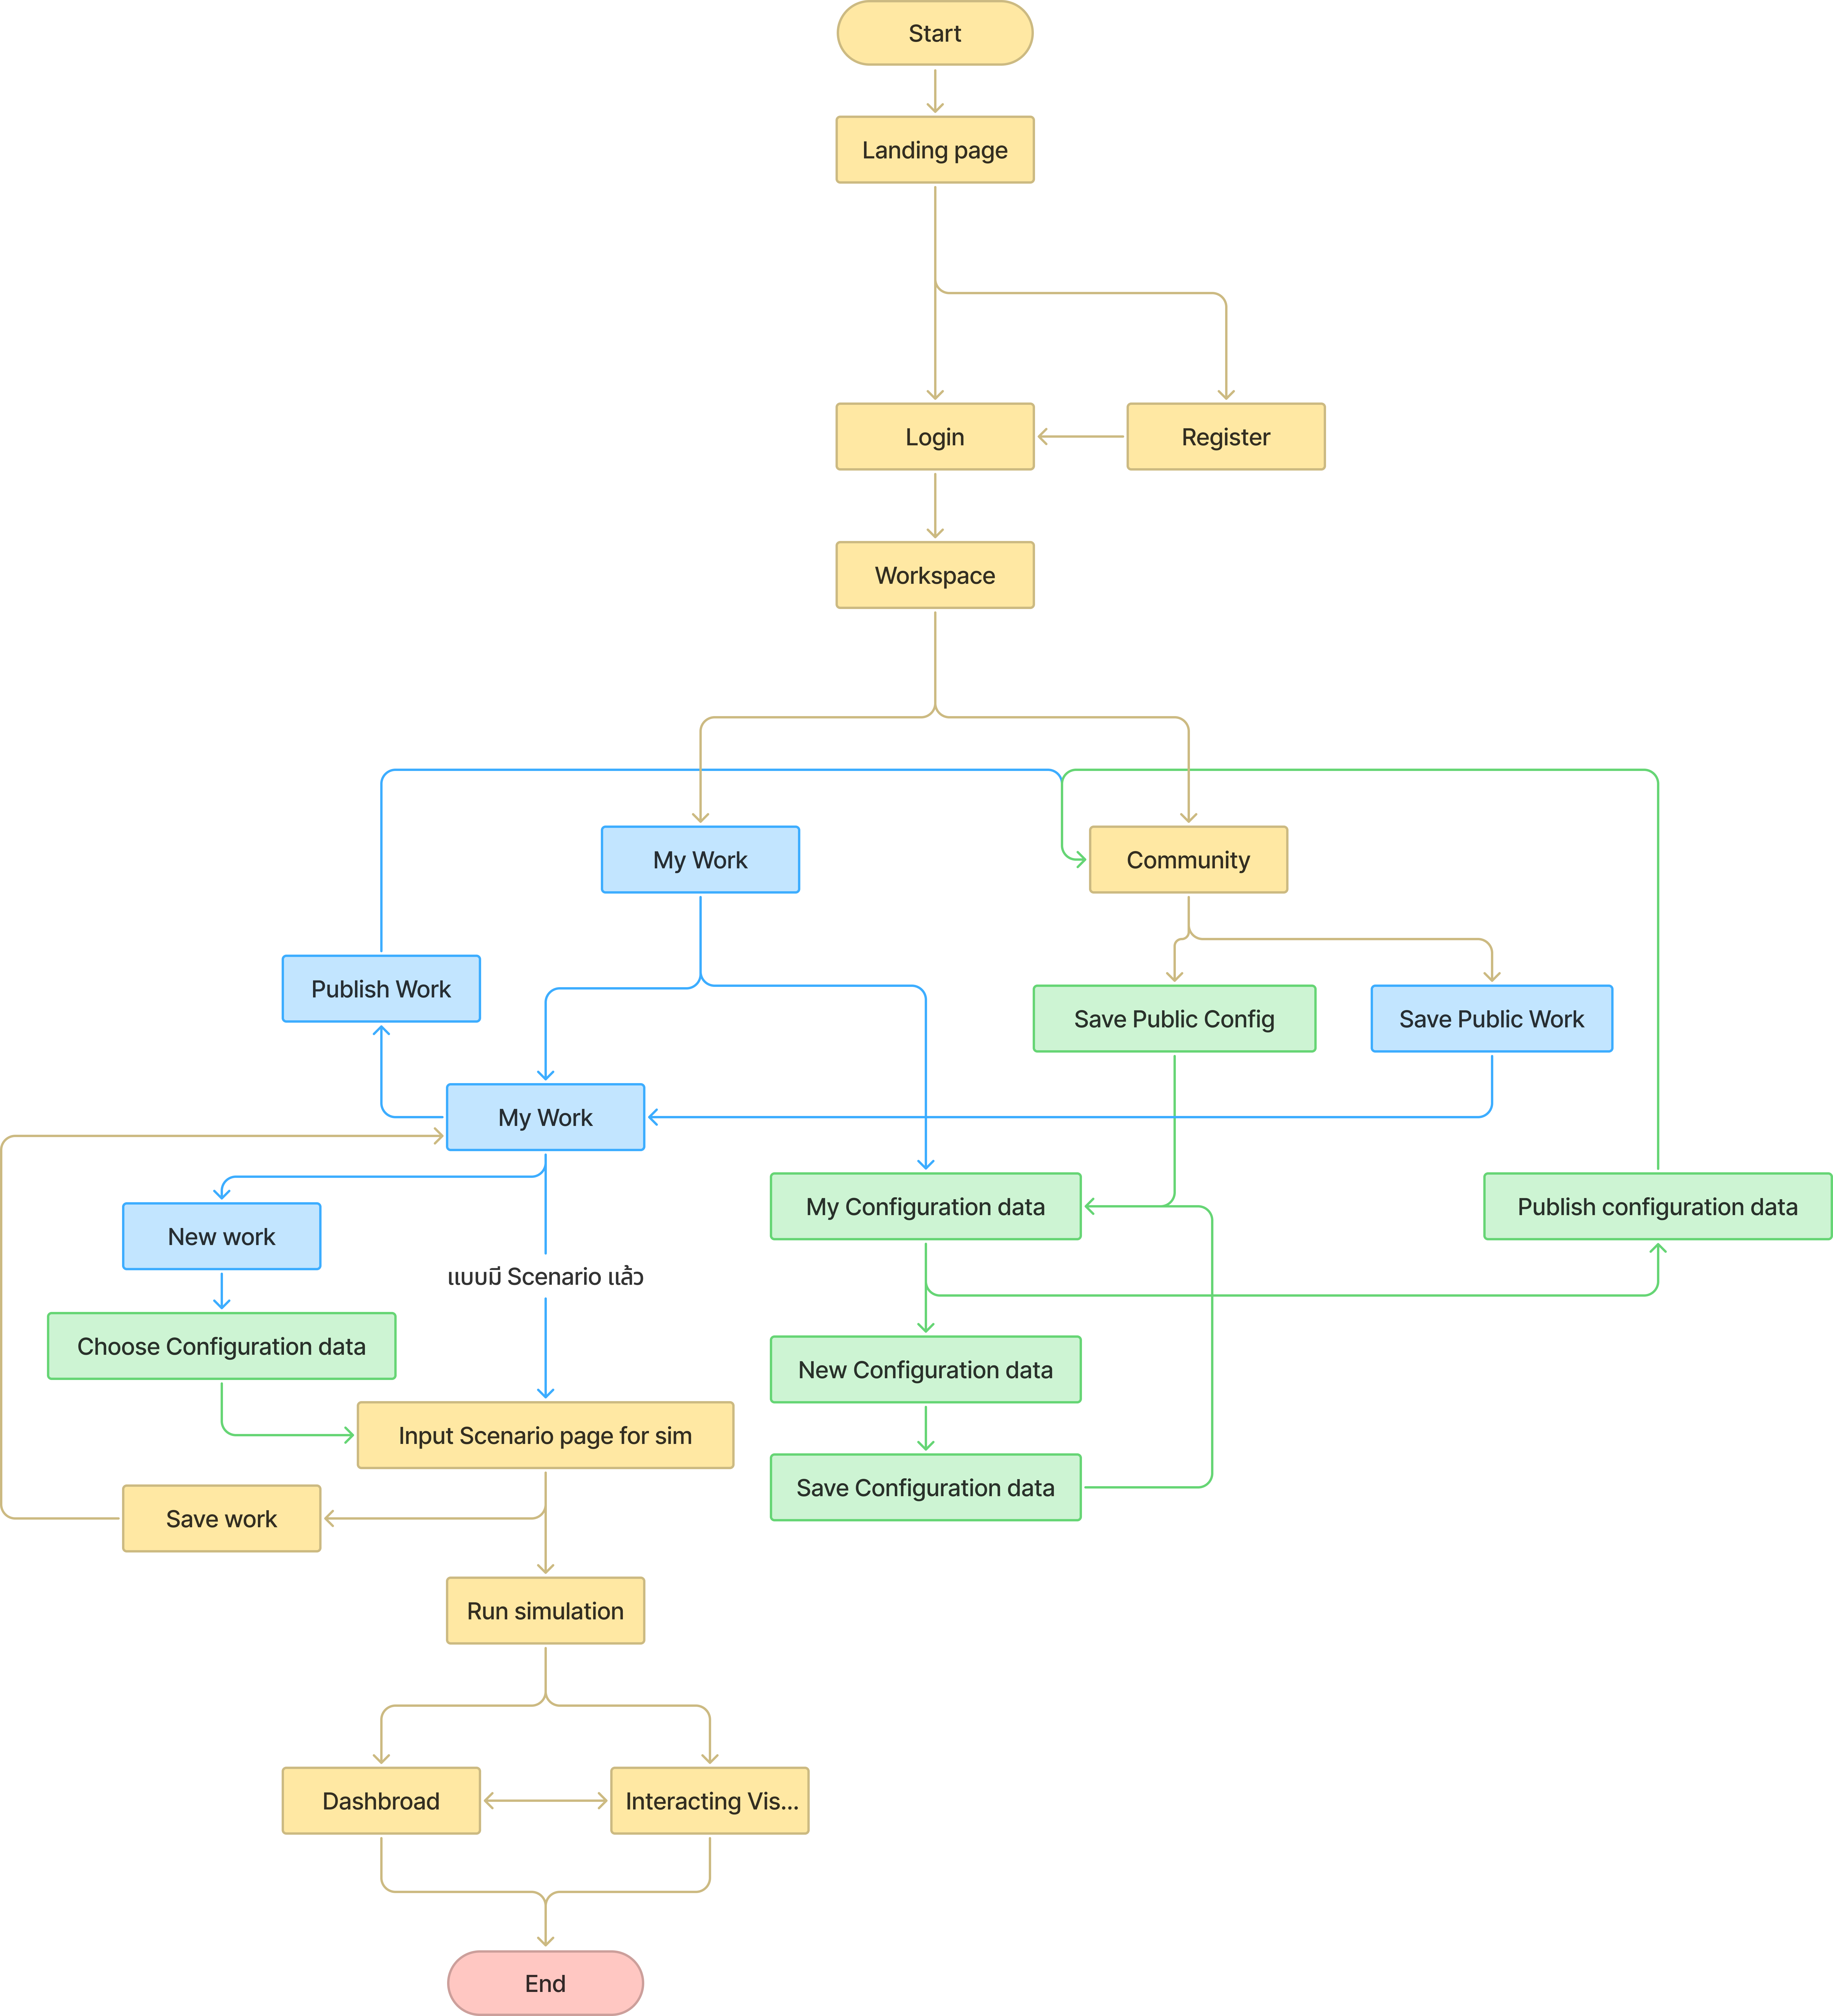
\includegraphics[width=\textwidth,height=0.9\textheight,keepaspectratio]{User_flow_-_login.png}
    \caption{user flow ของผู้ใช้ที่ลงทะเบียน}
    \label{fig:UserFlowRegistered}
    \end{figure}
    \newpage
    \item ผู้ใช้ที่ไม่ได้ลงทะเบียน (Guest Users / Unregistered Users)
        \begin{figure}[H]
    \centering
    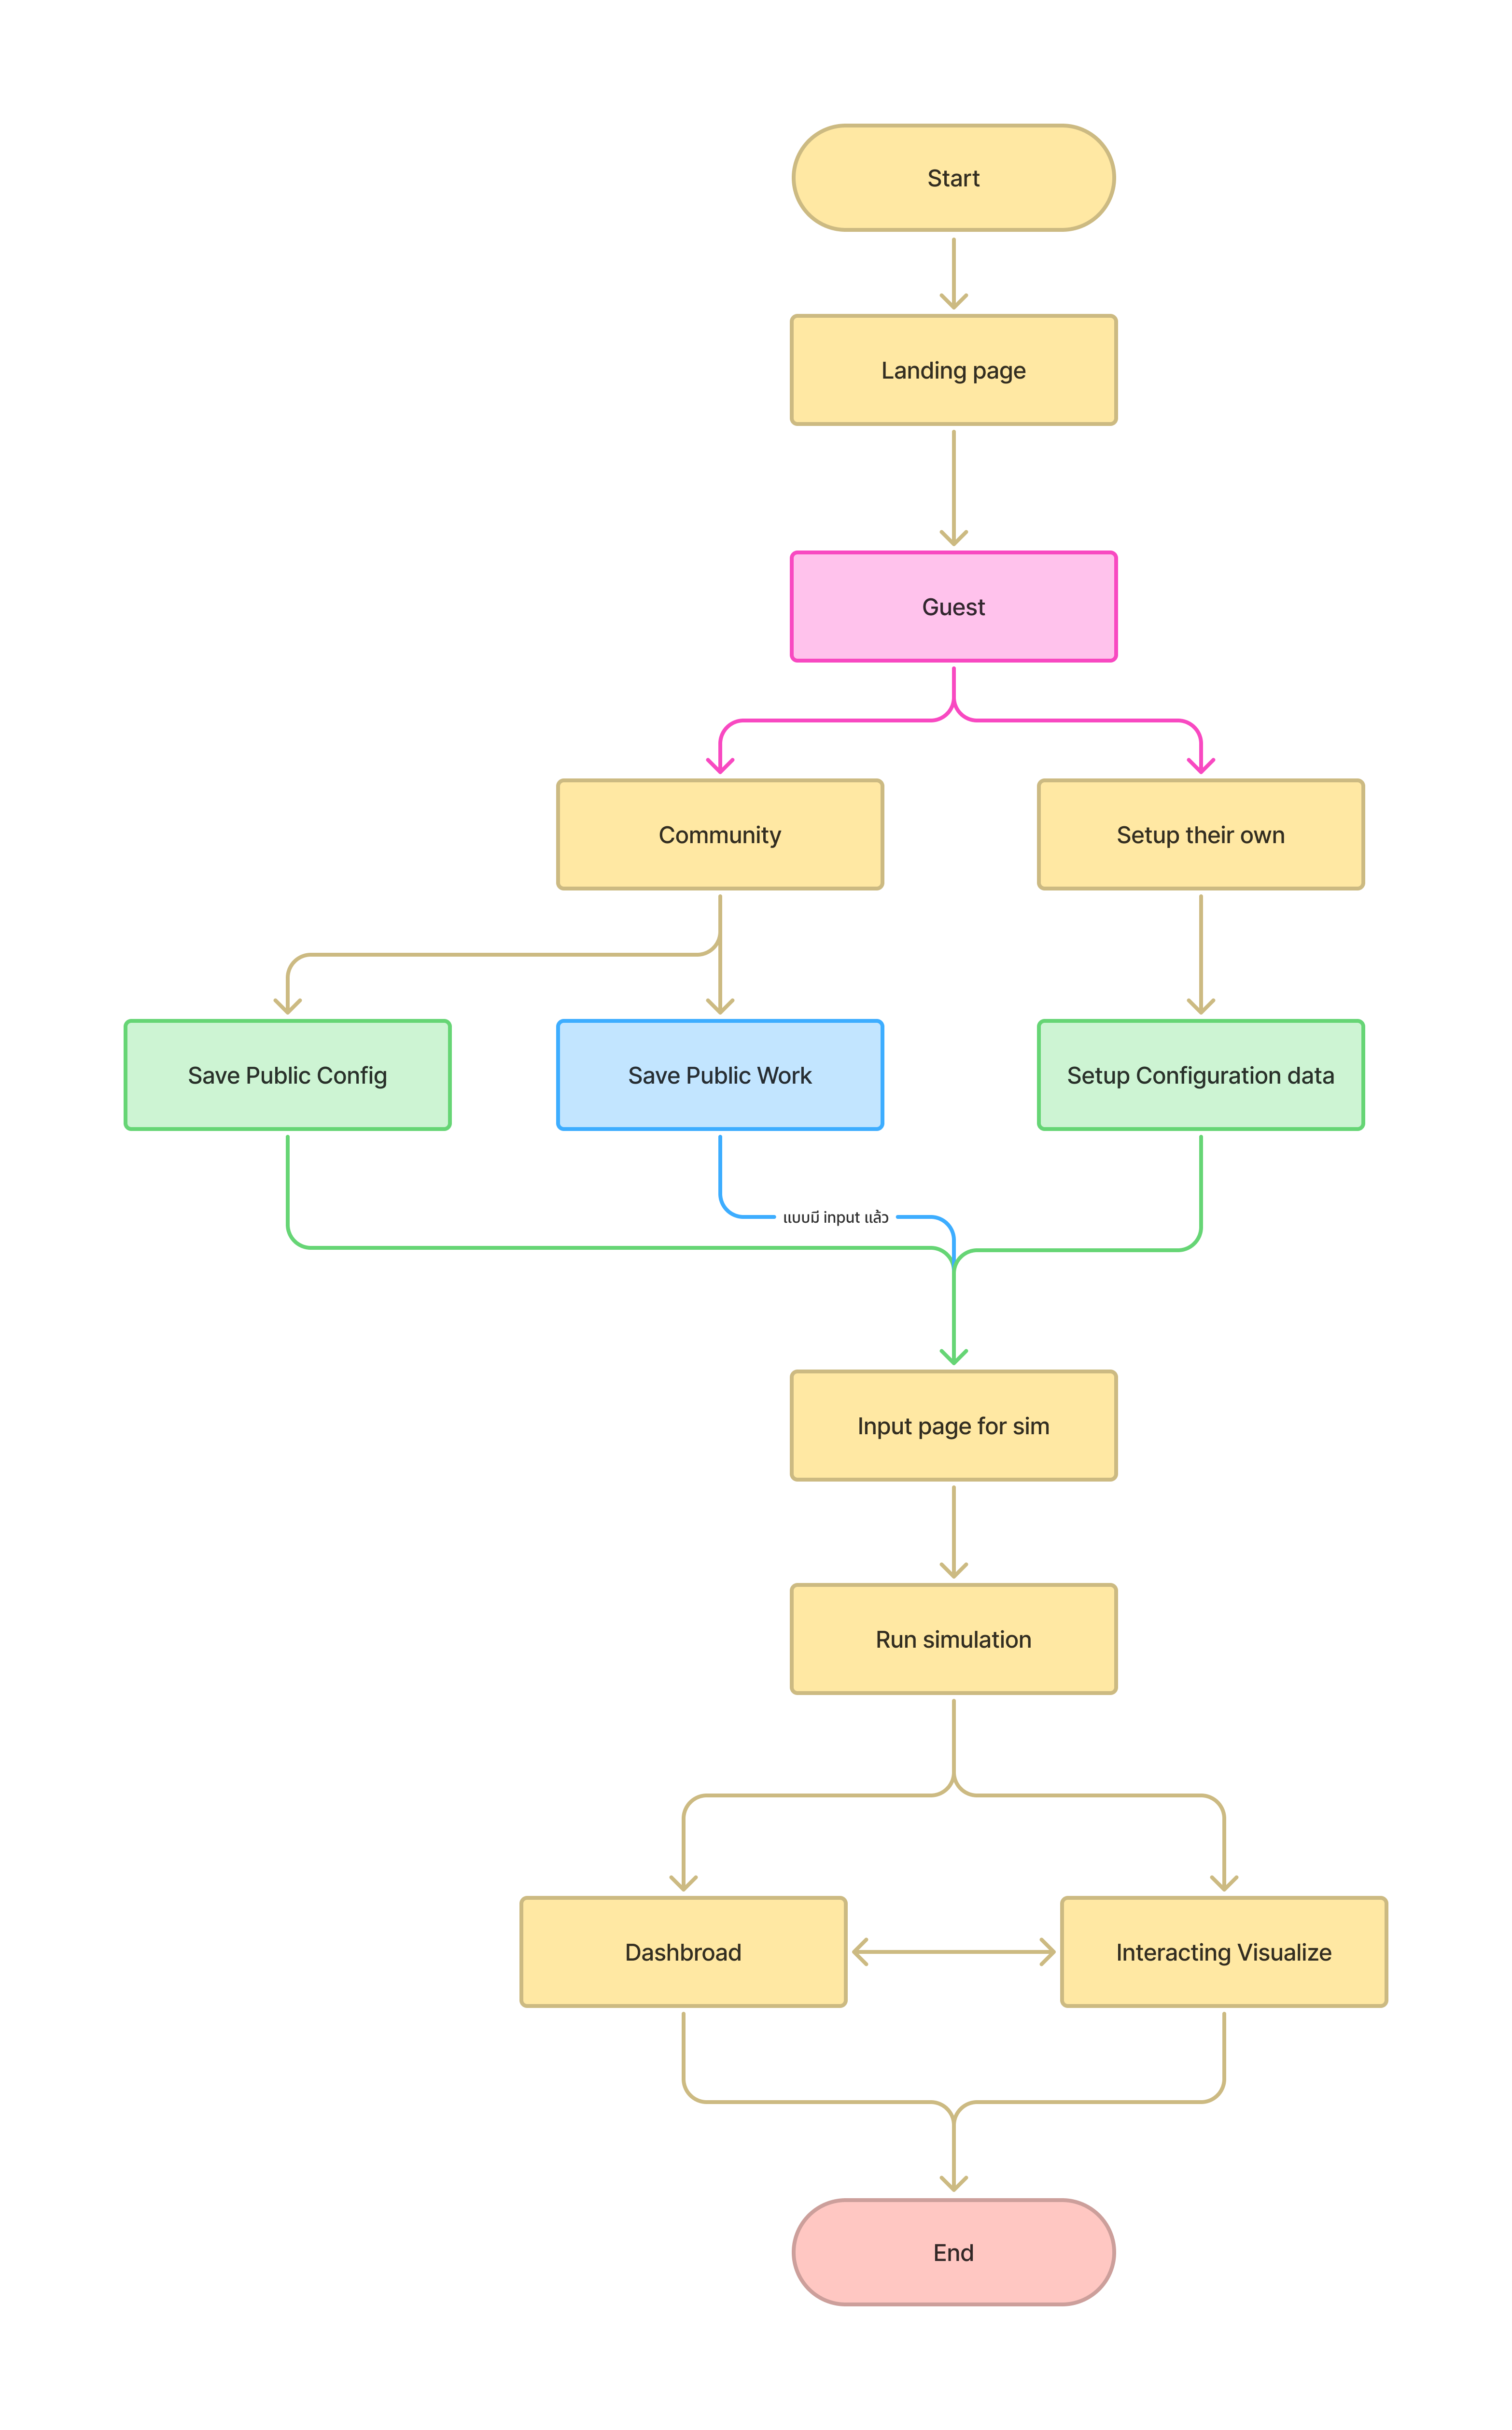
\includegraphics[width=\textwidth,height=0.9\textheight,keepaspectratio]{User_flow_-_guest.png}
    \caption{user flow  ของผู้ใช้ที่ไม่ได้ลงทะเบียน}
    \label{fig:UserFlowUnregistered}
    \end{figure}
\end{itemize}
\end{mypara}